\setcounter{section}{-1}
\section{Introduction}
\subsection{Projet 1}
Chaque année, les étudiants de deuxième bachelier ingénieur civil à l'ULB se doivent de 
présenter un rapport sur un système pouvant être chaotique afin d'acquérir une bonne 
compréhension de ce qu'est le chaos.\\

La branche des mathématiques étudiant ces phénomènes se nomme la théorie du chaos : 
\textit{"La théorie du chaos traite des systèmes dynamiques rigoureusement déterministes,
mais qui présentent un phénomène fondamental d'instabilité appelé « sensibilité aux conditions
initiales » qui, modulo une propriété supplémentaire de récurrence, les rend non prédictibilité
en pratique à « long » terme."} \cite{wiki}.\\

Cette définition implique qu'un système pouvant être relativement simple et modélisé de façon
déterministe par ses équations de mouvement peut se livrer à un comportement totalement différent
et imprévisible lors d'un changement des conditions initiales et ce même pour une faible
modification (de l'ordre de $10^{-3}$). Cette modification infinitésimale entraînant un résultat
chaotique est souvent nommée \textit{effet papillon}.\\

Ce rapport-ci a pour but d'étudier le mouvement chaotique d'un système régit par les équations de
mouvement suivantes\footnote{Ces équations sont obtenues à la section suivante. Les différents paramètres sont tous écrits dans les unités SI} \cite{projet1} :

\begin{equation}
\label{eq:a}
\left\{\begin{array}{l}
l\dfrac{d^2\theta}{dt^2} = -\dfrac{d^2x}{dt^2}\cos\theta - g\sin\theta\\
\ \ \dfrac{d^2x}{dt^2} = -\mu l\dfrac{d^2\theta}{dt^2}\cos\theta + \mu l\sin\theta\left(\dfrac{d\theta}{dt}\right)^2 - \kappa x
\end{array}\right.\ \ \ \ \ \ \ \ \ \ \ \ \ \ \ \text{où}\ \ \left\{\begin{array}{l}
\kappa = \frac{k}{m+M}\\
\mu = \frac{m}{m+M}
\end{array}\right.
\end{equation}\\
En fonctions des différents paramètres régissant l'équation du mouvement ($m, M, k$ et $l$) et
des conditions initiales (position et vitesse de $m$ et $M$), il nous faudra mettre en évidence
les valeurs de ces différents paramètres et conditions initiales pour lequel notre système se
comportera de façon chaotique.\\

\begin{center}
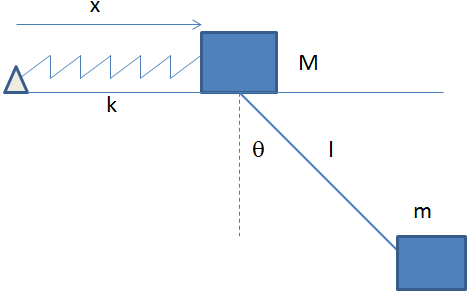
\includegraphics[scale=0.7]{intro/image1.png}
\captionof{figure}{Représentation schématique du projet 1}
\label{fig:projet1}
\end{center}


\newpage
\subsection{Équations du mouvement - Lagrange}
Les équations \textbf{REF} peuvent être obtenues en appliquant la méthode de Lagrange. Pour notre
système représenté la \autoref{fig:projet1}, nous pouvons avons deux degrés de liberté : $x$ et 
$\theta$.\\
Les énergies cinétiques des masses $m$ et $M$, respectivement $T_m$ et $T_M$ sont données par :

    \begin{equation}
        \left\{\begin{array}{l}
         T_m = \frac{1}{2}(\dot{x}^2 + 2l\dot{x}\dot{\theta}\cos\theta + l^2\dot{\theta}^2) \\
         T_M = \frac{1}{2}M\dot{x}^2
        \end{array}\right.
    \end{equation}
    
Il nous faut maintenant définir les potentiels de notre système. La masse $M$ ayant un potentiel 
constant, nous le définirons comme étant nul. Nous devons dès lors considérer uniquement le potentiel
du à la présence d'un ressort, $V_r$ ainsi que la potentiel gravitationnel de notre masse $m$, $V_m$ :


    \begin{equation}
        \left\{\begin{array}{l}
         V_k = \frac{1}{2}kx^2 \\
         V_m = -mgl\cos\theta
        \end{array}\right.
    \end{equation}

Notre lagrangien vaut ainsi : 

    \begin{equation}
        L = \frac{1}{2}(M\dot{x}^2 + \dot{x}^2 + 2l\dot{x}\dot{\theta}\cos\theta + l^2\dot{\theta}^2) -\frac{1}{2}kx^2 + mgl\cos\theta
    \end{equation}
    
    
Par la méthode de Lagrange, nous pouvons retrouver les équations de mouvement :

    \begin{equation}
        \left\{\begin{array}{ll}
         \frac{d}{dt}\left(\frac{\partial L}{\partial \dot{x}}\right) - \frac{\partial L}{\partial x} = 0 & \Leftrightarrow (m+M)\ddot{x} + ml(\ddot{\theta}\cos\theta - \dot{\theta}^2\sin\theta - kx = 0\\
         \frac{d}{dt}\left(\frac{\partial L}{\partial \dot{\theta}}\right) - \frac{\partial L}{\partial \theta} = 0 & \Leftrightarrow ml(\ddot{x}\cos\theta - \dot{x}\dot{\theta}\sin\theta + l\ddot{\theta}) - ml(-\dot{x}\dot{\theta}\sin\theta - g\sin\theta) = 0
        \end{array}\right.
    \end{equation}
    
En posant $\mu = \dfrac{m}{m+M}$ et $\kappa = \dfrac{k}{m+M}$, nous retrouvons les équations présentées
en \autoref{eq:a}.
